\documentclass{article}

\usepackage{arxiv}

\usepackage[utf8]{inputenc} % allow utf-8 input
\usepackage[T1]{fontenc}    % use 8-bit T1 fonts
\usepackage{lmodern}        % https://github.com/rstudio/rticles/issues/343
\usepackage{hyperref}       % hyperlinks
\usepackage{url}            % simple URL typesetting
\usepackage{booktabs}       % professional-quality tables
\usepackage{amsfonts}       % blackboard math symbols
\usepackage{nicefrac}       % compact symbols for 1/2, etc.
\usepackage{microtype}      % microtypography
\usepackage{lipsum}
\usepackage{graphicx}

\title{OLET5610 Report}

\author{
    Trent Henderson
   \\
     \\
   \\
  \texttt{\href{mailto:then6675@uni.sydney.edu.au}{\nolinkurl{then6675@uni.sydney.edu.au}}} \\
  }


% Pandoc citation processing
\newlength{\csllabelwidth}
\setlength{\csllabelwidth}{3em}
\newlength{\cslhangindent}
\setlength{\cslhangindent}{1.5em}
% for Pandoc 2.8 to 2.10.1
\newenvironment{cslreferences}%
  {}%
  {\par}
% For Pandoc 2.11+
\newenvironment{CSLReferences}[3] % #1 hanging-ident, #2 entry spacing
 {% don't indent paragraphs
  \setlength{\parindent}{0pt}
  % turn on hanging indent if param 1 is 1
  \ifodd #1 \everypar{\setlength{\hangindent}{\cslhangindent}}\ignorespaces\fi
  % set entry spacing
  \ifnum #2 > 0
  \setlength{\parskip}{#2\baselineskip}
  \fi
 }%
 {}
\usepackage{calc} % for calculating minipage widths
\newcommand{\CSLBlock}[1]{#1\hfill\break}
\newcommand{\CSLLeftMargin}[1]{\parbox[t]{\csllabelwidth}{#1}}
\newcommand{\CSLRightInline}[1]{\parbox[t]{\linewidth - \csllabelwidth}{#1}}
\newcommand{\CSLIndent}[1]{\hspace{\cslhangindent}#1}



\begin{document}
\maketitle

\def\tightlist{}


\begin{abstract}

\end{abstract}


\hypertarget{method}{%
\section{Method}\label{method}}

Time-series classification algorithms are typically benchmarked using
the Time Series Classification Repository, which contains 128 univariate
(i.e., values sampled uniformly in time) time-series classification
datasets/problems and 30 multivariate (i.e., for any time \(t\),
\(\mathbf{y}_{t} = (y_{1t},\ldots, y_{nt})\) describes \(n\)
realisations at time \(t\)) datasets (Anthony Bagnall and Keogh 2022).
Here, we focus on the univariate setting. Many algorithms developed
across the sciences have been evaluated across the standardised
univariate datasets provided in the repository, with black-box
algorithms typically outperforming competitors (Bagnall et al. 2017).
Given the growing need for algorithmic transparency in the sciences and
industry, the present research aims to explore the feasibility of a new
approach using one of the 128 datasets as a test case. Specifically,
this work aims to determine if using informative summary statistics
(known as ``features''), can be used to construct high performing
classification procedures that rival or outperform existing approaches
{[}Fulcher, Little, and Jones (2013); Fulcher (2017);
fulcherFeatureBasedTimeSeriesAnalysis2018{]}. Examples of such features
include properties of the time-series distribution of values,
autocorrelation structure, entropy, model-fit statistics, nonlinear
time-series analysis, stationarity, and many others (Fulcher and Jones
2014). At its core, feature-based time-series analysis reduces an time
series \(\times\) time matrix to a time series \(\times\) feature
matrix, which can then be used for statistical learning (such as
classification), using the interpretative values of time-series features
as inputs.

\hypertarget{dataset}{%
\subsection{Dataset}\label{dataset}}

The ``Wafer'' dataset in the Time Series Classification Repository
contains data relating to the fabrication of semi-conductor
microelectronics. The dataset comprises a collection of inline process
control measurements that were recorded from a range of sensors during
the manufacturing and processing of silicon wafers for semiconductor
fabrication. Each time series in the Wafer dataset represents the
measurements of one sensor during the processing of one wafer by one
tool. Labels for two classes are provided in the data: \emph{Normal} and
\emph{Abnormal}\footnote{\url{https://www.timeseriesclassification.com/description.php?Dataset=Wafer}}.
The goal of this problem is to predict class membership from the
time-series values. The dataset contains a pre-designated train-test
split, with 1000 samples in the train set (each of length \(T = 152\)),
and 6164 samples in the test set (each of length \(T = 152\)).

\hypertarget{algorithmic-approach}{%
\subsection{Algorithmic Approach}\label{algorithmic-approach}}

The approach in this work contains three stages: (i) extraction of
time-series features for each unique time series; (ii) dimensionality
reduction to obtain a reduced set of informative vectors; (iii)
classification using the dimensionality reduction results as inputs into
a random forest classifier. Features from two open-source feature sets
(\textbf{catch22} (Lubba et al. 2019; Henderson 2022a) and \textbf{Kats}
(Facebook Infrastructure Data Science 2021)) will be extracted using the
R package ``theft'' (Henderson 2022b). Given the \(T = 24\) length of
each time series, \textbf{catch22} will extract 24 features (as mean and
standard deviation are added to the standard 22 features) and
\textbf{Kats} will extract 40 features. This will produce a resulting
time series \(\times\) feature matrix of size 7164 \(\times\) 64. Given
the existence within-set redundancy (i.e., high absolute correlations
between features in a set) observed particularly for \textbf{Kats}
relative to \textbf{catch22} in previous work, dimensionality reduction
through principal components analysis (PCA) will then be applied to
substantially reduce the input matrix size for the classification
algorithm into a time series \(\times\) principal component matrix
(Henderson and Fulcher 2021). A threshold of 80\(\%\) cumulative
variance explained will be used to determine the principal components to
retain. Following the procedure of previous work (Ruiz et al. 2021), the
methodology will then train and evaluate the accuracy of the classifier
over 30 resamples of train-test splits, where each is seeded for
reproducibility and the first is always the pre-designated train-test
split in the data as it comes from the Time Series Classification
Repository. This will enable scientific inference of algorithmic
performance with uncertainty and facilitate a direct comparison with the
performance of existing methods.

Given the existence of the Time Series Classification Repository
(Anthony Bagnall and Keogh 2022) which holds the Wafer dataset (whose
sole purpose is to facilitate benchmarking of time-series classification
algorithms), it is expected that meaningful class separation will be
possible. The present research takes a novel approach of chaining
time-series feature extraction into dimensionality reduction techniques
into a classification algorithm --- an approach that has seen almost no
research attention to-date. As such, a primary goal of this work is to
understand the performance of this approach relative to current
benchmarks.

Given the high within-set redundancy (i.e., high absolute correlations
between features in a set) observed in previous work, it is hypothesised
that dimensionality reduction techniques will substantially reduce the
input matrix size for the classification algorithm from the original
time series \(\times\) feature matrix to a time series \(\times\)
principal component matrix (Henderson and Fulcher 2021). Further, it is
also hypothesised that using the time series \(\times\) principal
component matrix as input to a classification algorithm (i.e., random
forest classifier) will not result in a substantial reduction in
classification performance compared to using the time series \(\times\)
feature matrix.

\hypertarget{results}{%
\section{Results}\label{results}}

Prior to substantative analysis, exploratory data analysis was
performed. A sample of three time series from each class (\emph{Normal}
and \emph{Abnormal}) is displayed in Figure @ref(fig:tsplots). To the
eye, some small, but noticeable differences in temporal dynamics and
shape are visible between the classes, which suggests that
classification based on temporal properties (i.e, ``features'') is a
feasible approach.

\begin{figure}
\centering
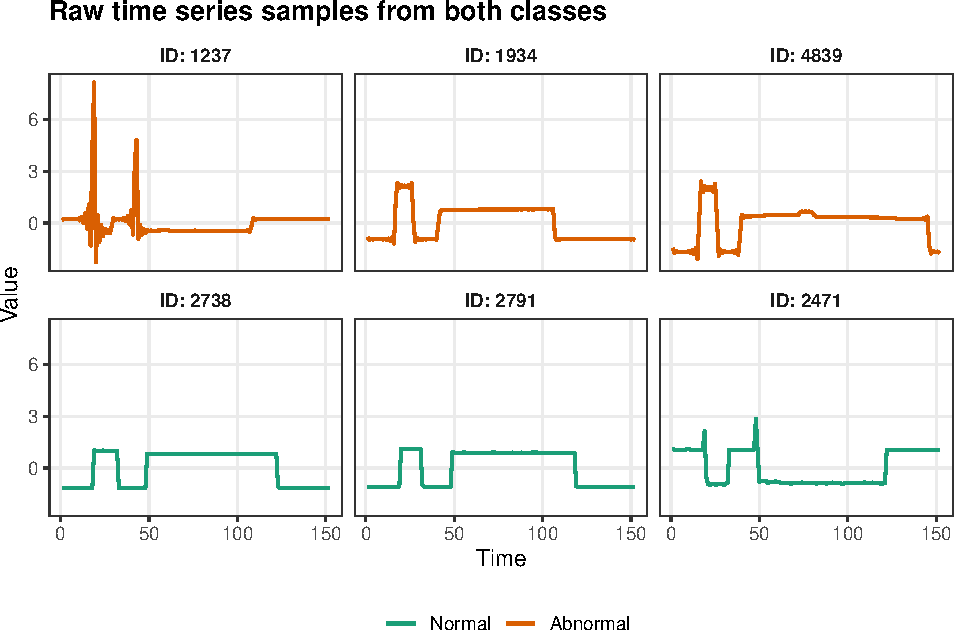
\includegraphics{olet5610_report_files/figure-latex/tsplots-1.pdf}
\caption{Raw time-series plots of three randomly selected time series
from each class (\(Normal\) and \(Abnormal\)) in the Wafer dataset.
Small differences in temporal dynamics are visible.}
\end{figure}

\hypertarget{dimensionality-reduction}{%
\subsection{Dimensionality reduction}\label{dimensionality-reduction}}

Time-series features were computed from two sets (\textbf{catch22} and
\textbf{Kats}) on all time series, which produced a time series
\(\times\) feature matrix of size 7164 \(\times\) 64. This matrix is
large, which increases computation time for classification algorithms
and increases complexity of model interpretation and evaluation. To
reduce this complexity, a principal components analysis was performed.
The dataset meets the assumptions of PCA, as multicollinearity between
time-series features was a reason for conducting the analysis, and there
are sufficient samples to adequately perform PCA as the \(7164:64\)
\(samples:variables\) ratio exceeds the \(20:1\) recommendation for PCA
(Osborne and Costello 2019).

Figure @ref(fig:eigenplots) plots a visual summary of the PCA. Panel
\textbf{(A)} plots the percentage of variance explained for the top
eight principal components (PC) which explain 80\(\%\) of the variance.
\(PC 1\) explains \(37.5\%\) of the variance, but there is a steep drop
off following this component, with \(PC 2\) explaining \(15.6\%\) of the
variance. Panel \textbf{(B)} plots cumulative variance explained for the
eight retained PCs. The first four PCs explain two-thirds of the
variance in the dataset. Panel \textbf{(C)} plots the eigenvalues of the
eight PCs. All eight PCs exceed the \(\lambda = 1\) threshold for the
Kaiser criterion of PC retention (Kaiser 1960).

\begin{figure}
\centering
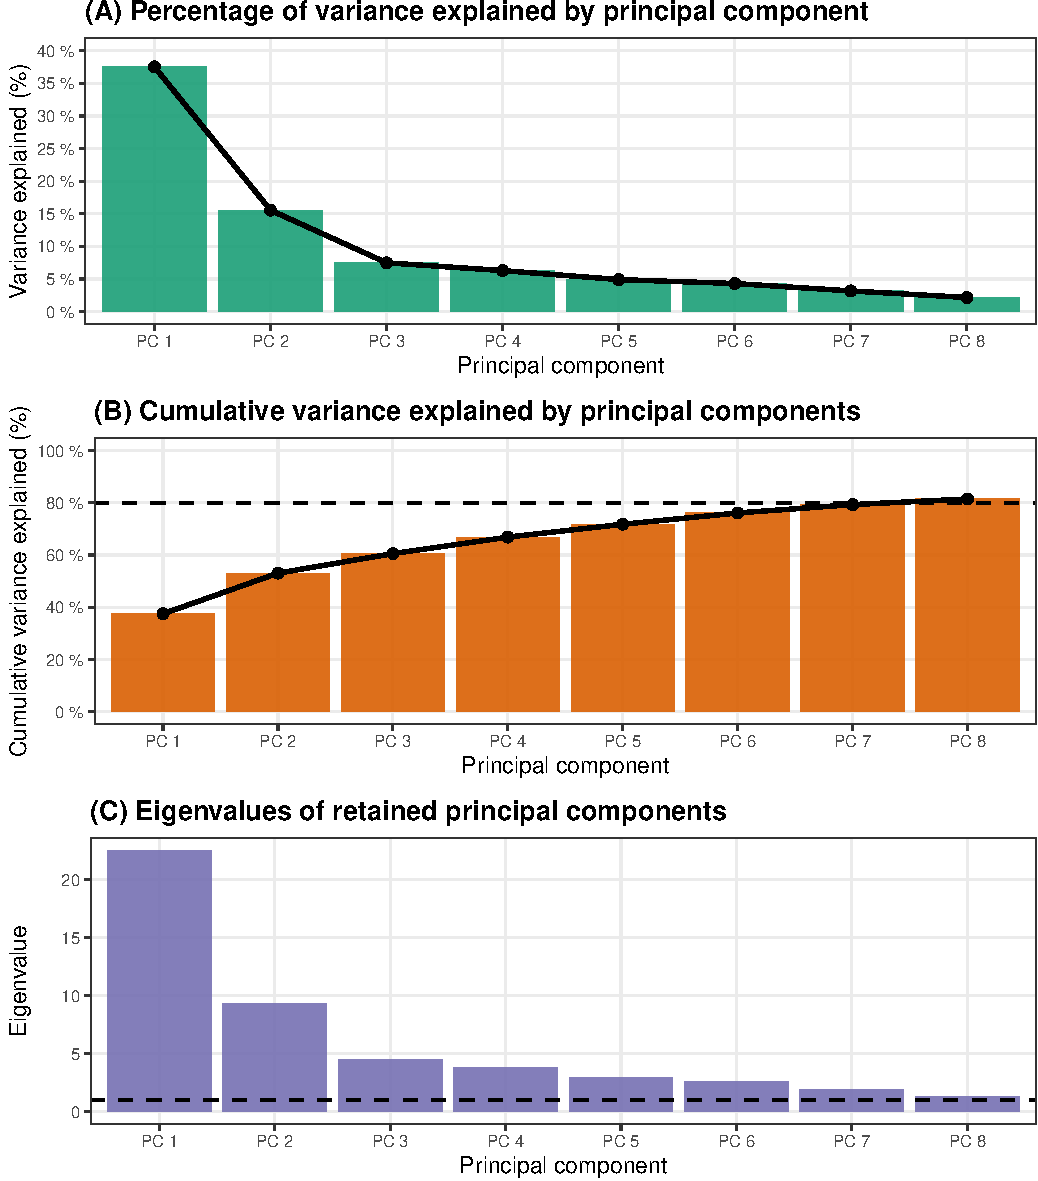
\includegraphics{olet5610_report_files/figure-latex/eigenplots-1.pdf}
\caption{Summary of eight retained principal components. (A) Percentage
of variance explained is plotted in descending order for each of the
retained principal components. (B) Cumulative variance explained is
plotted for each of the retained principal components. An 80\%
cumulative variance threshold was selected to determine the principal
components to retain which returned the eight plotted here (from the
original 64). (C) Eigenvalues of the eight retained principal components
are plotted in descending order. All retained components also exceed the
\(\lambda = 1\) cutoff for the Kaiser criterion.}
\end{figure}

Loadings for each of the 64 time-series features (variables) on the
eight PCs is presented in Figure @ref(fig:loadplot). Patterns are
evident across the PCs, such as the strong loading of time-series
features associated with properties of the autocorrelation and partial
autocorrelation function onto \(PC 1\), and histogram-based statistics
onto \(PC 3\). This plot gives us interpretable and informative insight
into the relative behaviour of the time-series features extracted from
the Wafer dataset.

\begin{figure}
\centering
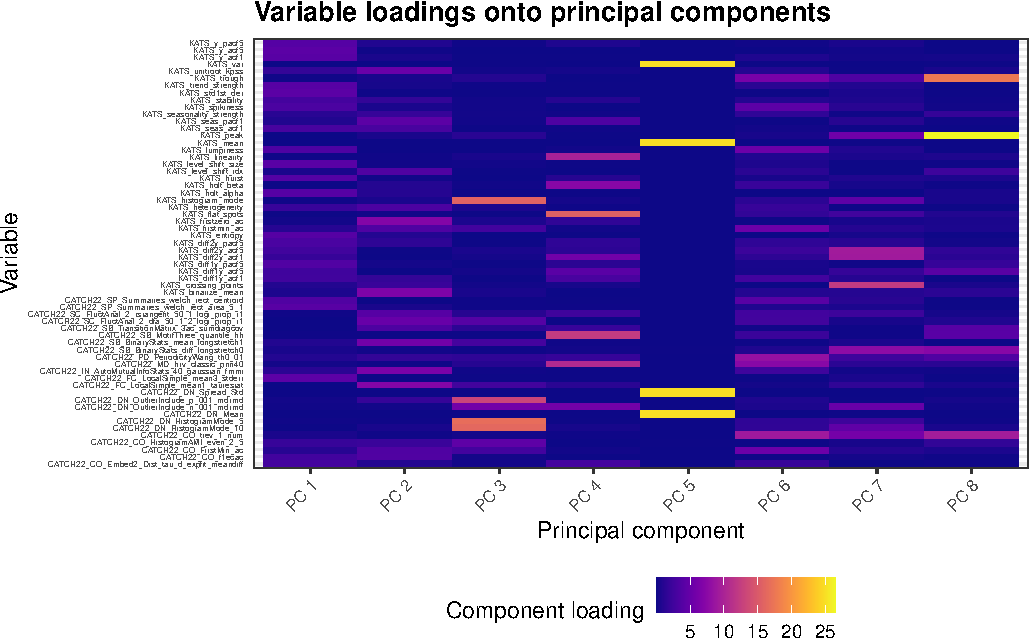
\includegraphics{olet5610_report_files/figure-latex/loadplot-1.pdf}
\caption{Loadings of each variable onto the eight retained principal
components.}
\end{figure}

Prior to modelling, the PCA was distilled into an even lower dimensional
space of just two dimensions to understand if class differences could be
ascertained with just the two PCs which explain the most variance in the
data (a collective \(53.1\%\)). This is displayed in Figure
@ref(fig:biplot)). There is considerable overlap between the \(Normal\)
and \(Abnormal\) classes in the two-dimensional space, suggesting the
additional six principal components are likely needed for accurate
classification.

\begin{figure}
\centering
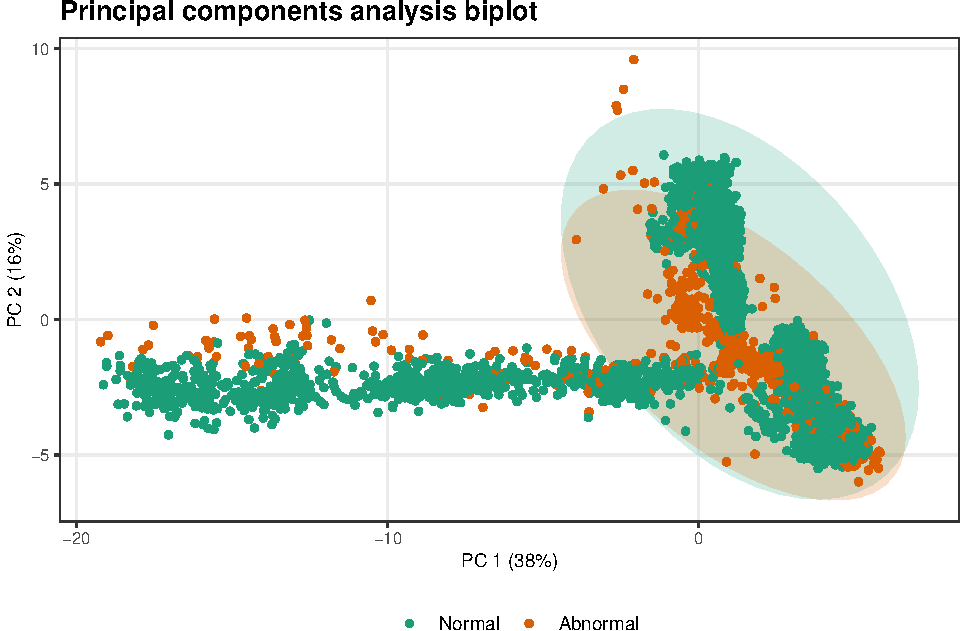
\includegraphics{olet5610_report_files/figure-latex/biplot-1.pdf}
\caption{Principal components analysis biplot. The first principal
component (positioned along the \(x\)-axis) explains \(37.5\%\) of the
variance in the Wafer dataset. The second principal component
(positioned along the \(y\)-axis) explains \(15.6\%\) of the variance in
the Wafer dataset.}
\end{figure}

\hypertarget{time-series-classification}{%
\subsection{Time-series
classification}\label{time-series-classification}}

The time series \(\times\) principal component matrix (7164 \(\times\)
8) was passed as input into a random forest classifier using the
\textbf{caret} package in R (Kuhn 2020) over 30 resamples, where the
first sample was the pre-designated train-test split from the Time
Series Classification Repository. Mean balanced classification accuracy
across the resamples was \(99.08\% (SD=0.19\%)\) and is compared to
previous benchmarks (Bagnall et al. 2017) in Table @ref(tab:comptable).
The benchmark algorithms include collective of transformation-based
ensembles (COTE), shaepelet transform (ST), bag of SFA symbols (BOSS),
elastic ensemble (EE), dynamic time warping (DTW), time series forest
(TSF), time series bag of features (TSBF), learned pattern (LPS), and
move-split-merge (MSM). The current approach, while marginally
outperformed by the other algorithms, demonstrates classification
performance that can be considered to be on-par with complex, more
black-box models despite only using eight principal components as an
input to a random forest classifier.

\begin{table}

\caption{\label{tab:comptable}Comparison of mean classification accuracy results on the Wafer dataset between the current approach and existing benchmarks. Performance differences are minimal between all approaches, with each algorithm achieving $\>99\%$ accuracy.}
\centering
\begin{tabular}[t]{l|l}
\hline
Algorithm & Mean Accuracy\\
\hline
ST & 100\%\\
\hline
COTE & 99.9\%\\
\hline
BOSS & 99.9\%\\
\hline
EE & 99.7\%\\
\hline
TSF & 99.7\%\\
\hline
DTW & 99.6\%\\
\hline
TSBF & 99.6\%\\
\hline
MSM & 99.6\%\\
\hline
LPS & 99.5\%\\
\hline
Current approach & 99.1\%\\
\hline
\end{tabular}
\end{table}

To understand the performance of the approach in the current work, we
examine the machinery of the random forest models. Understanding
relative variable importance can shed a deeper light into random forest
models to aid interpretability. Variable importance ranks for each
variable (principal components) across the 30 resamples are plotted in
Figure @ref(fig:impranks). \(PC 4\) (comprised of mostly symbolic
features, such as those associated with entropy of small-set
probabilities, flat spots, and proportion of magnitudes that exceed a
threshold over the standard deviation) is the most important variable
across all 30 resamples for predicting class (\(Normal\) versus
\(Abnormal\)). The performance of \(PC 4\) is further demonstrated in
Figure @ref(fig:impdists) which plots the mean \(\pm1SD\) of variable
importance values across the 30 resamples. On average, \(PC 4\) exhibits
variable importance of a factor of 5.5 higher than any other variable.

\begin{figure}
\centering
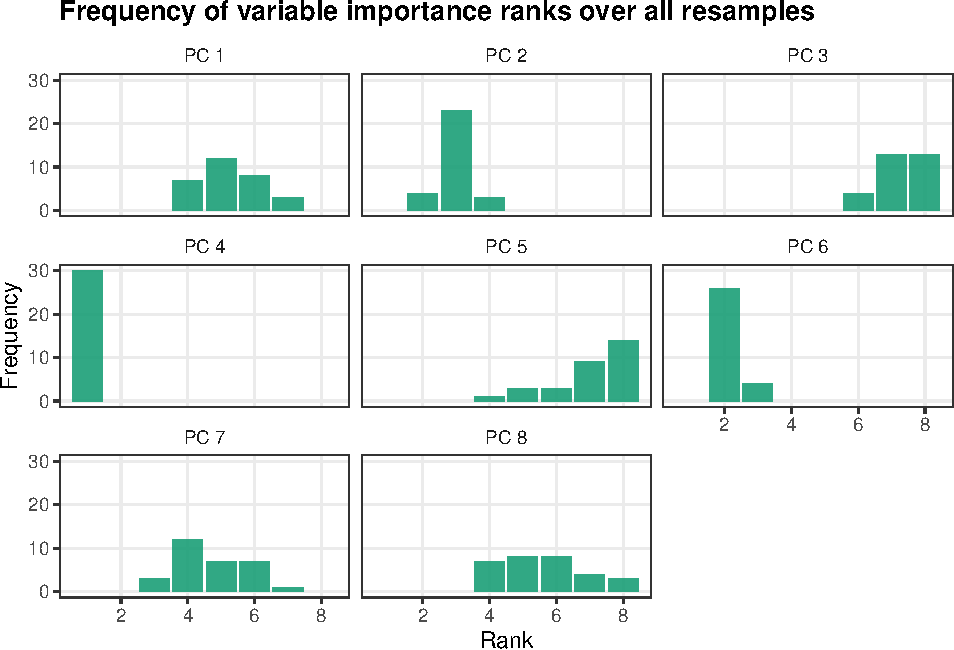
\includegraphics{olet5610_report_files/figure-latex/impranks-1.pdf}
\caption{Frequency of ranks over all resamples are plotted for each
principal component used as a predictor in the models. \(PC 4\) is the
most important variable across all 30 resamples for predicting class
(\(Normal\) versus \(Abnormal\)).}
\end{figure}

\begin{figure}
\centering
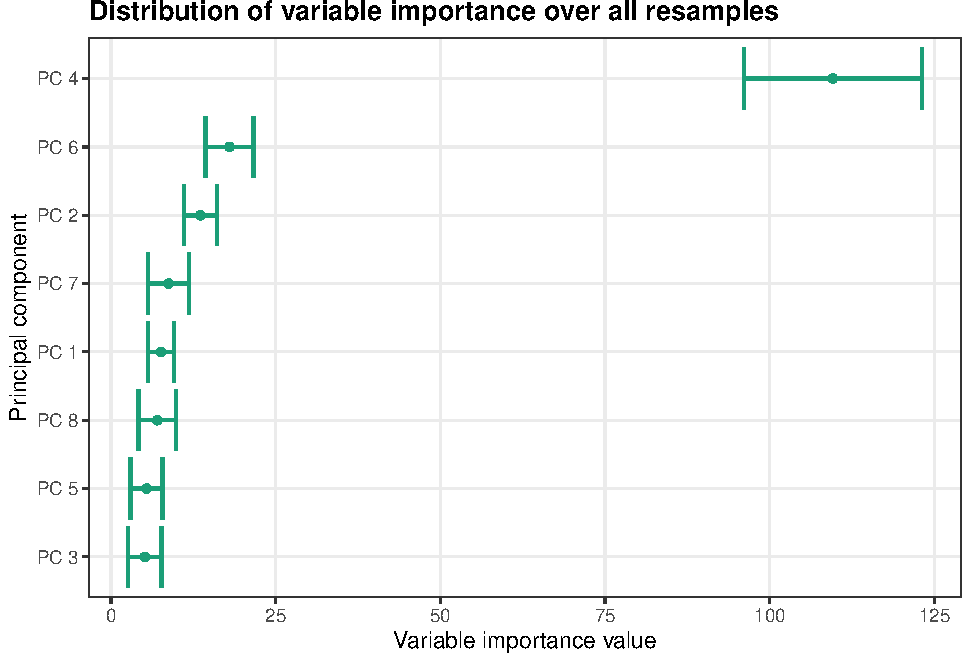
\includegraphics{olet5610_report_files/figure-latex/impdists-1.pdf}
\caption{Mean variable importance \(\pm\) 1SD is plotted for each
principal component used as predictors in the models. \(PC 4\)
demonstrates the highest mean variable importance values by a factor of
5.5 over the next highest component (\(PC 6\)).}
\end{figure}

\hypertarget{references}{%
\section*{References}\label{references}}
\addcontentsline{toc}{section}{References}

\hypertarget{refs}{}
\begin{CSLReferences}{1}{0}
\leavevmode\hypertarget{ref-UEA_UCR_Repo}{}%
Anthony Bagnall, William Vickers, Jason Lines, and Eamonn Keogh. 2022.
{``The UEA \& UCR Time Series Classification Repository.''}
\href{https://www.timeseriesclassification.com}{www.timeseriesclassification.com}.

\leavevmode\hypertarget{ref-bagnallGreatTimeSeries2017}{}%
Bagnall, Anthony, Jason Lines, Aaron Bostrom, James Large, and Eamonn
Keogh. 2017. {``The Great Time Series Classification Bake Off: A Review
and Experimental Evaluation of Recent Algorithmic Advances.''}
\emph{Data Mining and Knowledge Discovery} 31 (3): 606--60.
\url{https://doi.org/10.1007/s10618-016-0483-9}.

\leavevmode\hypertarget{ref-Kats}{}%
Facebook Infrastructure Data Science. 2021. {``Kats.''}
\url{https://facebookresearch.github.io/Kats/}.

\leavevmode\hypertarget{ref-fulcherFeaturebasedTimeseriesAnalysis2017}{}%
Fulcher, Ben D. 2017. {``Feature-Based Time-Series Analysis.''}
\emph{arXiv:1709.08055 {[}Cs{]}}, October.
\url{http://arxiv.org/abs/1709.08055}.

\leavevmode\hypertarget{ref-fulcherHighlyComparativeFeaturebased2014}{}%
Fulcher, Ben D., and Nick S. Jones. 2014. {``Highly Comparative
Feature-Based Time-Series Classification.''} \emph{IEEE Transactions on
Knowledge and Data Engineering} 26 (12): 3026--37.
\url{https://doi.org/10.1109/TKDE.2014.2316504}.

\leavevmode\hypertarget{ref-fulcherHighlyComparativeTimeseries2013}{}%
Fulcher, Ben D., Max A. Little, and Nick S. Jones. 2013. {``Highly
Comparative Time-Series Analysis: The Empirical Structure of Time Series
and Their Methods.''} \emph{Journal of The Royal Society Interface} 10
(83): 20130048. \url{https://doi.org/10.1098/rsif.2013.0048}.

\leavevmode\hypertarget{ref-Rcatch22}{}%
Henderson, Trent. 2022a. \emph{Rcatch22: Calculation of 22 CAnonical
Time-Series CHaracteristics}.

\leavevmode\hypertarget{ref-theft}{}%
---------. 2022b. \emph{Theft: Tools for Handling Extraction of Features
from Time Series}. \url{https://hendersontrent.github.io/theft/}.

\leavevmode\hypertarget{ref-hendersonEmpiricalEvaluationTimeSeries2021}{}%
Henderson, Trent, and Ben D. Fulcher. 2021. {``An {Empirical Evaluation}
of {Time-Series Feature Sets}.''} In \emph{2021 {International
Conference} on {Data Mining Workshops} ({ICDMW})}, 1032--38.
\url{https://doi.org/10.1109/ICDMW53433.2021.00134}.

\leavevmode\hypertarget{ref-Kaiser1960}{}%
Kaiser, Henry F. 1960. {``The Application of Electronic Computers to
Factor Analysis.''} \emph{Educational and Psychological Measurement} 20
(1): 141--51. \url{https://doi.org/10.1177/001316446002000116}.

\leavevmode\hypertarget{ref-caret}{}%
Kuhn, Max. 2020. \emph{Caret: Classification and Regression Training}.
\url{https://CRAN.R-project.org/package=caret}.

\leavevmode\hypertarget{ref-lubbaCatch22CAnonicalTimeseries2019}{}%
Lubba, Carl H., Sarab S. Sethi, Philip Knaute, Simon R. Schultz, Ben D.
Fulcher, and Nick S. Jones. 2019. {``Catch22: {CAnonical Time-series
CHaracteristics}.''} \emph{Data Mining and Knowledge Discovery} 33 (6):
1821--52. \url{https://doi.org/10.1007/s10618-019-00647-x}.

\leavevmode\hypertarget{ref-osborneSampleSizeSubject2019}{}%
Osborne, Jason, and Anna Costello. 2019. {``Sample Size and Subject to
Item Ratio in Principal Components Analysis.''} \emph{Practical
Assessment, Research, and Evaluation} 9 (1).
\url{https://doi.org/10.7275/ktzq-jq66}.

\leavevmode\hypertarget{ref-ruizGreatMultivariateTime2021}{}%
Ruiz, Alejandro Pasos, Michael Flynn, James Large, Matthew Middlehurst,
and Anthony Bagnall. 2021. {``The Great Multivariate Time Series
Classification Bake Off: A Review and Experimental Evaluation of Recent
Algorithmic Advances.''} \emph{Data Mining and Knowledge Discovery} 35
(2): 401--49. \url{https://doi.org/10.1007/s10618-020-00727-3}.

\end{CSLReferences}

\bibliographystyle{unsrt}
\bibliography{references.bib}


\end{document}
